Until now, our analysis has assumed that in order to find a torrent and begin the download process a node must directly identify any node currently participating in that torrent. This need not be the case. Rather, to find a torrent, we could first discover the torrent's tracking data. The tracking data will contain a list of nodes thought to be participating in the torrent, these nodes can be used to initiate the download. This is, of course, analogous to the original BitTorrent protocol's torrent-discovery-via-trackers mechanism. To accomplish this in a unstructured P2P environment, we need a mechanism by which each peer indexes a random, non-disjoint subset of torrent tracking data. Given this mechanism, we can apply PAC search on the collection of tracking data, where each torrent's tracking data is equivalent to a document. The success of PAC search is then dependent on the distribution of torrent tracking data, rather than the distribution of the torrents themselves. 

In Section~\ref{sec:extension:indexing} we first introduce the modification to the BitTorrent protocol that enables peers to index a random, non-disjoint subset of torrent tracking data. Section~\ref{sec:extension:model} provides a mathematical model of our extension. Section~\ref{sec:extension:discussion} then analyses the distribution of torrent tracking data and the associated performance of PAC search.

\subsection{Indexing}\label{sec:extension:indexing}

    The ability of a PAC search system to return successful results is influenced by these two, controllable, factors: (i) the distribution of documents across the network, $r_i$, and (ii) the number of nodes contacted per query, $z$. The distribution of torrents over nodes discovered in Section~\ref{sec:measurement} prevents the vast majority of torrents from being discovered no matter how large $z$. Thus, as well as modifying $z$, we must also alter the distribution of the tracking data, $r_i$. From an information retrieval perspective, we do not need to replicate the file, or any pieces of the file, to more nodes. Rather, we need more nodes to be aware of where the torrent can be downloaded from. We need nodes in the network to store the torrent's unique ID and the list of peers participating in the torrent (tracking data), {\em even if the node itself is not participating in the torrent}. To this end, we introduce an index at each node that contains details of previously received requests. When a node is queried for a torrent that it does not own, the queried node stores details of the request in its index, i.e. storing the torrent's unique ID alongside the details of the node that made the request. If the queried node receives any future requests for that torrent, it can now respond with details of a node that it believes to own the torrent. When the querying node receives such a response, it can the contact these nodes directly. Thus, when a node performs a {\em search} it issues one or more queries for a torrent, until such time as a query is successful. A {\em query} consists of a node sending a request to $z$ randomly sampled nodes in the network. Each repeated query for the same torrent selects $z$ different nodes. A successful query is one that results in at least one successful request. A {\em request} consists of a querying node sending the desired torrent's infohash to one of the $z$ random nodes. The queried node responds with either a list of nodes it believes are participating in the torrent, or an empty list. A successful request returns a list of actively participating nodes; nodes that are online and that are downloading or uploading the torrent's data. A unsuccessful request returns either an empty list, or a list of nodes that are not participating in the torrent, e.g. because they have left the network.

\subsection{Model}\label{sec:extension:model}

    When querying a fixed number of random nodes, $z$, the probability of a successful query is now determined by (i) the number of nodes participating in the torrent, and (ii) the number of nodes indexing the torrent's tracking data, $r_i$. Given our proposed modification to the BitTorrent protocol, the more queries the network receives for a torrent, the more that torrent's tracking data is replicated, and the easier it becomes to find. At any point in time, $t$, the number of nodes indexing a torrent, $r(t)$, depends on (i) the total number of requests made for the torrent at $t$, and (ii) the number of nodes left in the network that were already indexing the torrent. In \cite{Crosby2007} the authors observe that in 95\% of the queries they made of the BitTorrent DHT, 20\% of the contacted nodes were not available. We therefore assume that of the $r(t-1)$ nodes indexing the torrent at time $t-1$, $0.8r(t-1)$ are available at time $t$. In \cite{Guo2007} the authors create a fluid model of BitTorrent networks, using that the node arrival rate at a torrent follows an exponentially decreasing rule with time: $\lambda_0e^{-\frac{t}{\tau}}$. Here, $\lambda_0$ indicates the arrival rate at $t=0$ and $\tau$ gives the attenuation parameter of the distribution. We can use this model to calculate how many nodes first index the torrent at each point in time. For each search made for the torrent a number of requests will be made, the total number of requests required depends on the existing replication. We use the expected value of a geometric distribution to model this: $zP(d_i)^{-1}$. Some of the nodes contacted will be indexing the torrent already, contacting these nodes does not increase the replication of the tracking data but does signify a successful query. We use the expected value of a hyper-geometric distribution to model the proportion of contacted nodes that did not index the torrent already: $(1-r(t-1)n^{-1})$. Eqn~\ref{eq:replication} combines the above to give a recursive definition of the number of nodes that are indexing a torrent at time $t$.

    \begin{equation}
        r(t) = \lambda_0e^{-\frac{t}{\tau}}(1 + z(1-r(t-1)n^{-1})P(d_i)^{-1})+0.8r(t-1)
        \label{eq:replication}
    \end{equation}

    The recursive definition of $r(t)$ requires that a base value be set for $r(1)$. Conceptually, $r(1)$ is the number of nodes indexing the torrent when the torrent is brand new, i.e. before any searches have been made for it. The value for $r(1)$ can be controlled by the single authoring node by the use of dummy queries. Each query publicises the new torrent and can be used to bootstrap tracking data around the network.

\subsection{Discussion}\label{sec:extension:discussion}

    The probability of a successful query is controlled by $z$ and $r(t)$. When a node wishes to query for a torrent's tracking data they must issues $z$ requests. If the replication of the tracking data were known then $z$ could be selected to provide a desired probability of success. Unfortunately, the only point in time when the replication is known is at $t=1$, when the author is bootstrapping the tracking data. At this early stage the author can pick a replication that provides a desired probability of success for a desired $z$. After this time, the replication will depend on the number of searches made for the torrent and the speed at which nodes leave the network. Figure~\ref{fig:required_z} shows our model's prediction of the value for $z$ required to provide a desired probability of successful query at a given point in time. Here we have assumed a torrent that has a peer arrival distribution of $50e^{\frac{-t}{50}}$. The replication at $t=1$ has been set at a value that requires $z=100$ in order to provide the desired probability of successful query. Over time the required $z$ value increases as the replication of tracking data falls. Figure~\ref{fig:replication} shows the decrease in replication over time. Nodes search for the torrent at an exponentially decreasing rate, early in the torrent's lifetime the replication is high because many nodes are making requests for that torrent. Later in the torrent's lifetime, far fewer searches are being performed for the torrent and so the replication decreases with the network churn. Consequently, $z$ has to increase to maintain the probability of success. For this torrent, the average search requires $z=143$, $z=270$, $z=340$, and $z=396$ for probability of success $P(d_i)=0.5$, $P(d_i)=0.8$, $P(d_i)=0.9$, and $P(d_i)=0.95$ respectively.

    \begin{figure}[t]
        \centering
        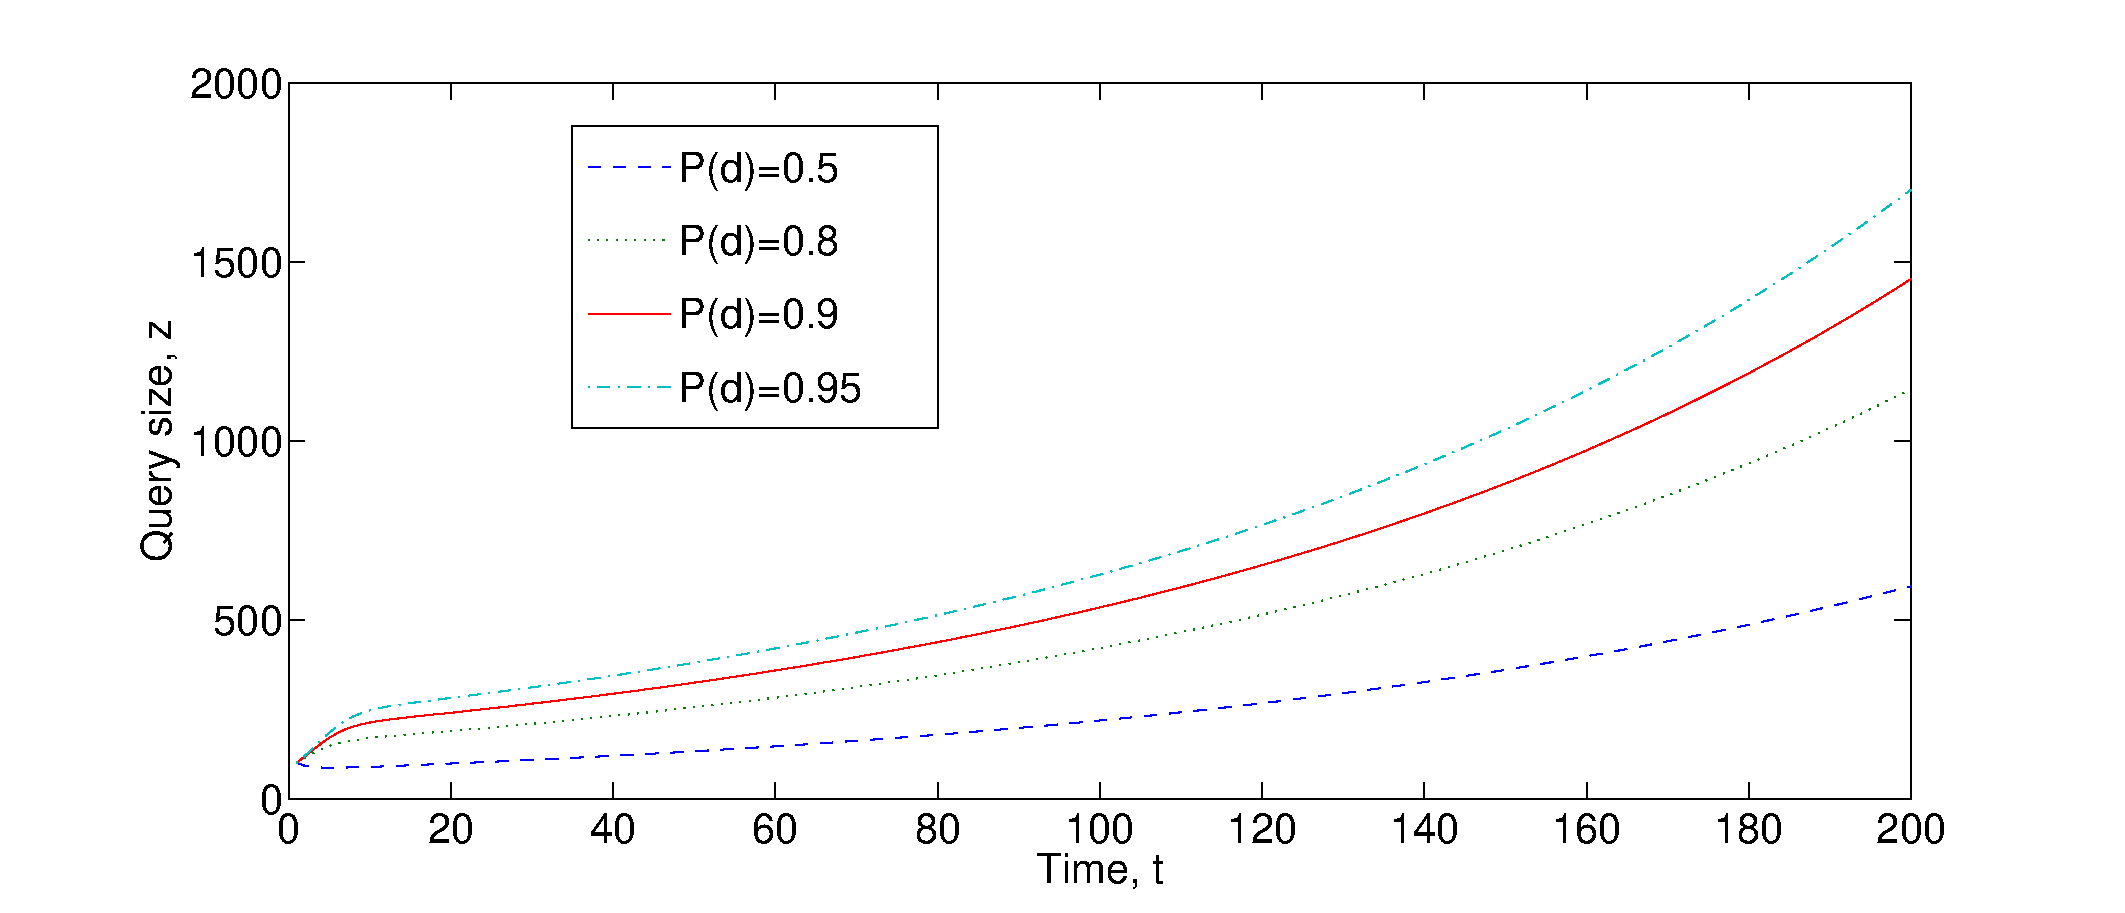
\includegraphics[width=0.5\textwidth]{Images/RequiredZ.eps}
        \caption{The number of nodes to query, $z$, over time, $t$, required to achieve a given probability of successful query}
        \label{fig:required_z}
    \end{figure}

    \begin{figure}[t]
        \centering
        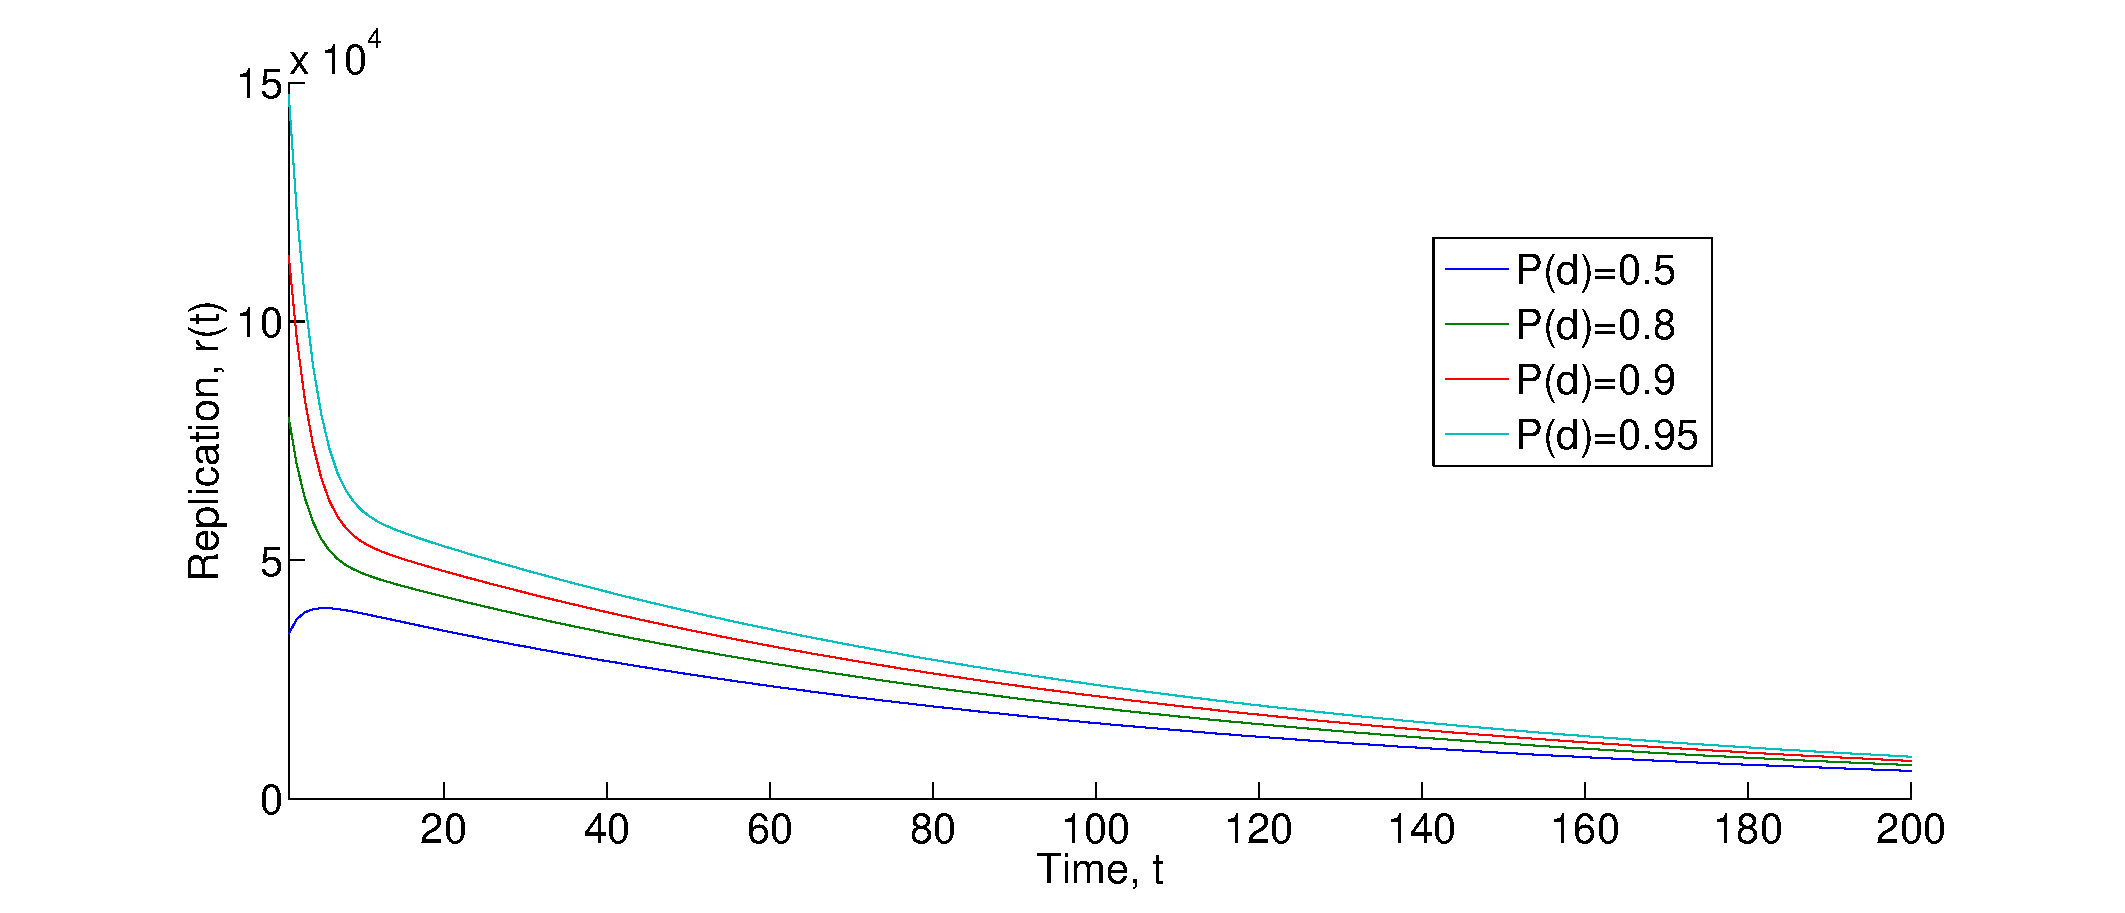
\includegraphics[width=0.5\textwidth]{Images/Replication.eps}
        \caption{The number of nodes that are indexing a torrent, $r(t)$, over time, $t$.}
        \label{fig:replication}
    \end{figure}
